\section{Introduction}
In this short tutorial you will get a brief overview of our Moflon tool. We give you some examples to show you the main features of our tool. When you have finished this tutorial, you will have an idea what you can do with this tool.
\newline
But first we recomend that you work through Part I for installation instructions.


%---------------------------------------------------------------------------------------------------
\subsection{Seting up your workspace}
After you have worked through Part I and your installation was hopefully successful, open the \texttt{Install, configure and deploy Moflon} button, go to \texttt{Install Workspace} and select the \texttt{Handbook Example (Final)} (Fig.~\ref{demo_workspace}). Now you have all necessary files to work through this tutorial.

\begin{figure}[htbp]
	\centering
  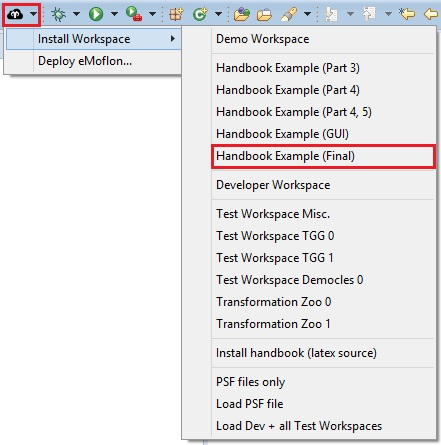
\includegraphics[width=0.8\textwidth]{eclipse_worcspace_final}
	\caption{Checking out the final workspace} 
	\label{demo_workspace} 
\end{figure}

%---------------------------------------------------------------------------------------------------
\subsection{Running example}
In this tutorial we use a running example to demonstrate the main possibilities of our tool. So for a better understanding, we will now explain the scenario.
\begin{itemize}
\item First, open the \texttt{Leitners\-Learning\-Box.eap} file in \texttt{Leitners\-Learning\-Box} (Fig.~\ref{eclipse_open_eap}). Enterprise Architect (EA) should open.

\begin{figure}[htbp]
	\centering
  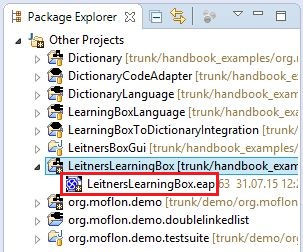
\includegraphics[width=0.5\textwidth]{eclipse_select_learningbox}
	\caption{Open \texttt{Leitners\-Learning\-Box.eap} file} 
	\label{eclipse_open_eap} 
\end{figure}

\item While this tutorial we use two metamodels. For this reason we have two class diagrams, \texttt{LearningBoxLanguage} and \texttt{DictionaryLanguage}. For a better understanding open both like in Fig.~\ref{ea_select_classdiagrams}.

  \begin{figure}[htbp]
	\centering
  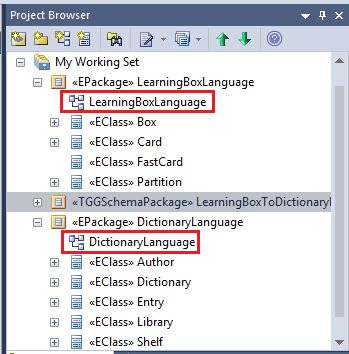
\includegraphics[width=0.5\textwidth]{ea_select_classdiagrams}
	\caption{Open the class diagrams \texttt{Learning\-Box\-Language} and \texttt{Dictionary\-Language}} 
	\label{ea_select_classdiagrams} 
\end{figure}

\end{itemize}

First have a look at \texttt{DictionaryLanguage} (Fig.~\ref{ea:classdiagram_DictionaryLanguage}). It  describes a simple library. In a library you have different authors and shelfes, which contains the dictionary with some entries. This is how you imagine a library. So every element of a library is here realized by a own class. 

\begin{figure}[htbp]
	\centering
  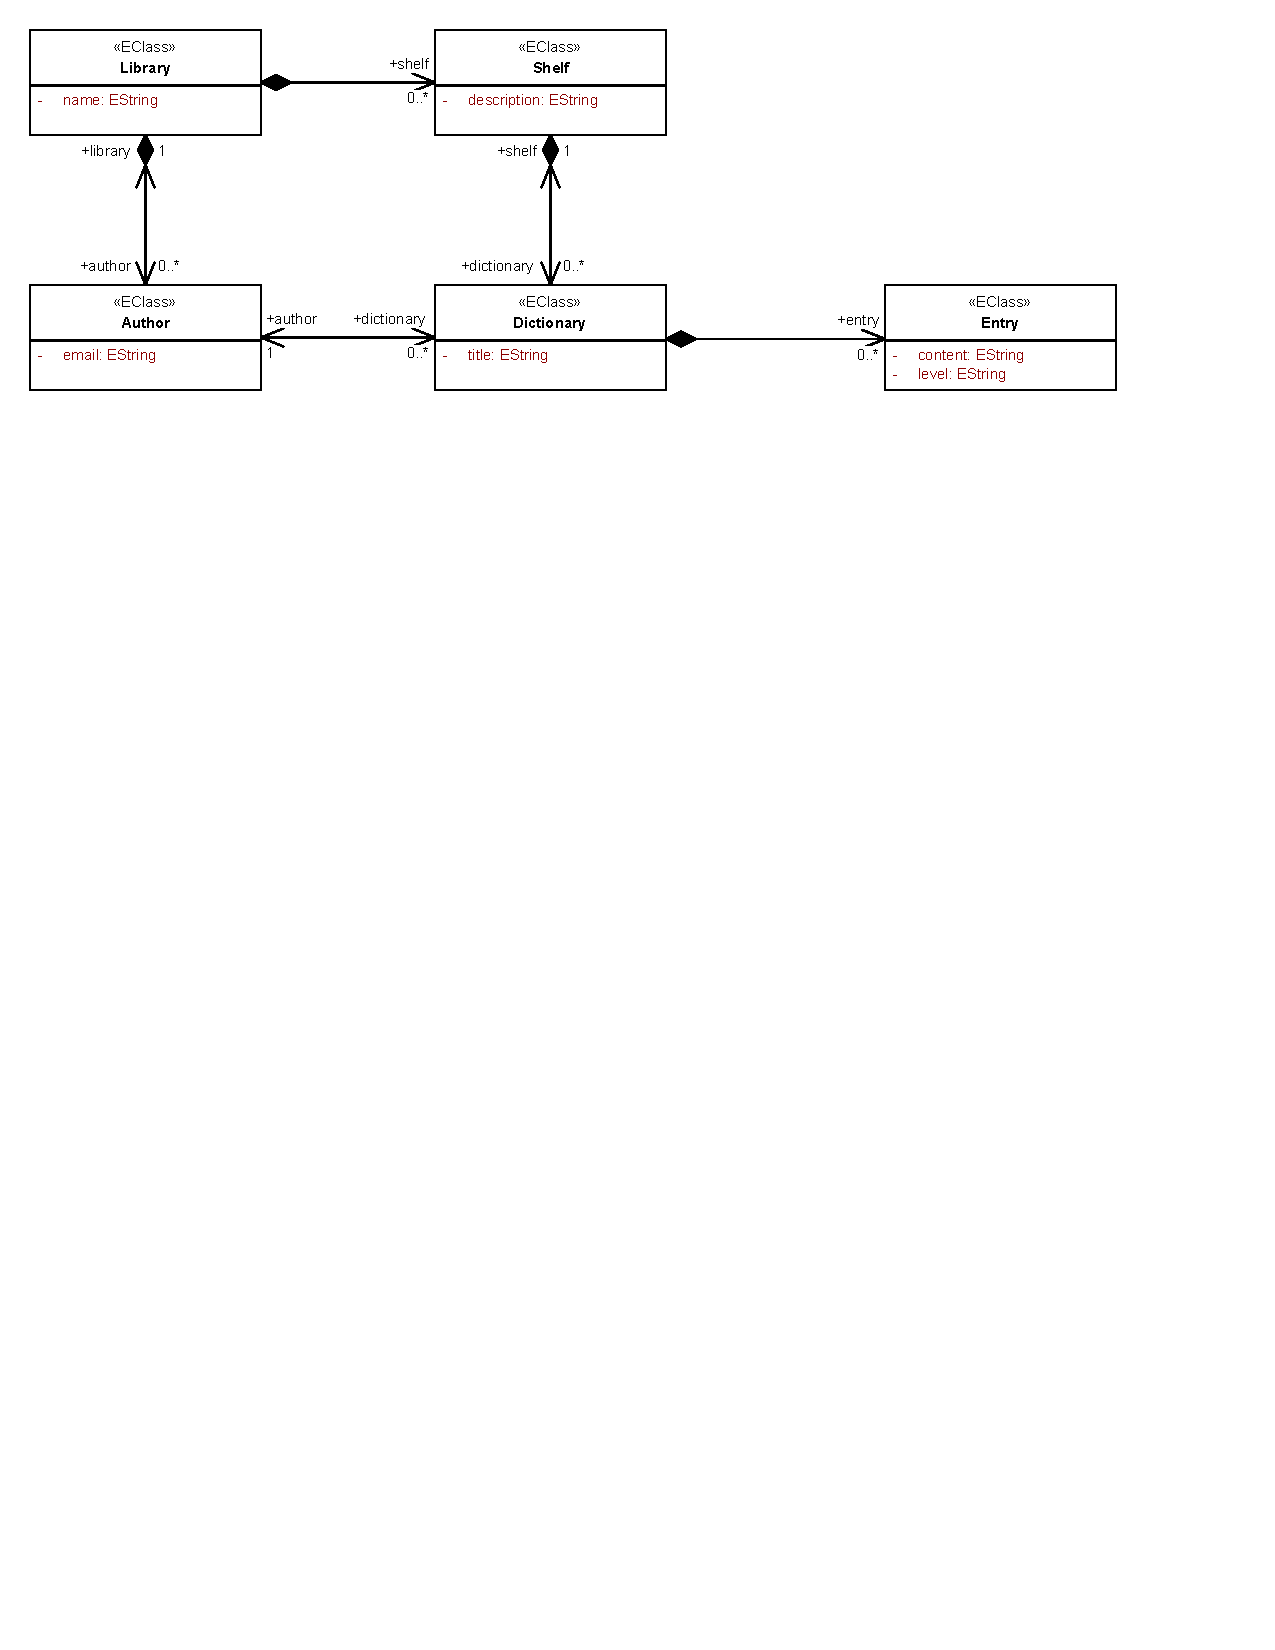
\includegraphics[width=1.2\textwidth]{Dictionary_classdiagram}
	\caption{Classdiagram of \texttt{Dictionary\-Language}} 
	\label{ea:classdiagram_DictionaryLanguage} 
\end{figure}

The other metamodel \texttt{Learning\-Box\-Language} describes the Leitners Learning box (Fig.~\ref{ea:classdiagram_LearningBoxLanguage}). Leitners Learning box is a file card based learning system for vocabularies. It consists of a box with a certain number of partitions. In the partition are cards with vocabularies on it. How the cards are moved between the different partitions is for this tutorial unimportant. But if you want to know more about it, work through Part II of our handbook.
\newline
In the classdiagram you can see that each element of the Learning box is also realized by an own class like before.

\begin{figure}[htbp]
	\centering
  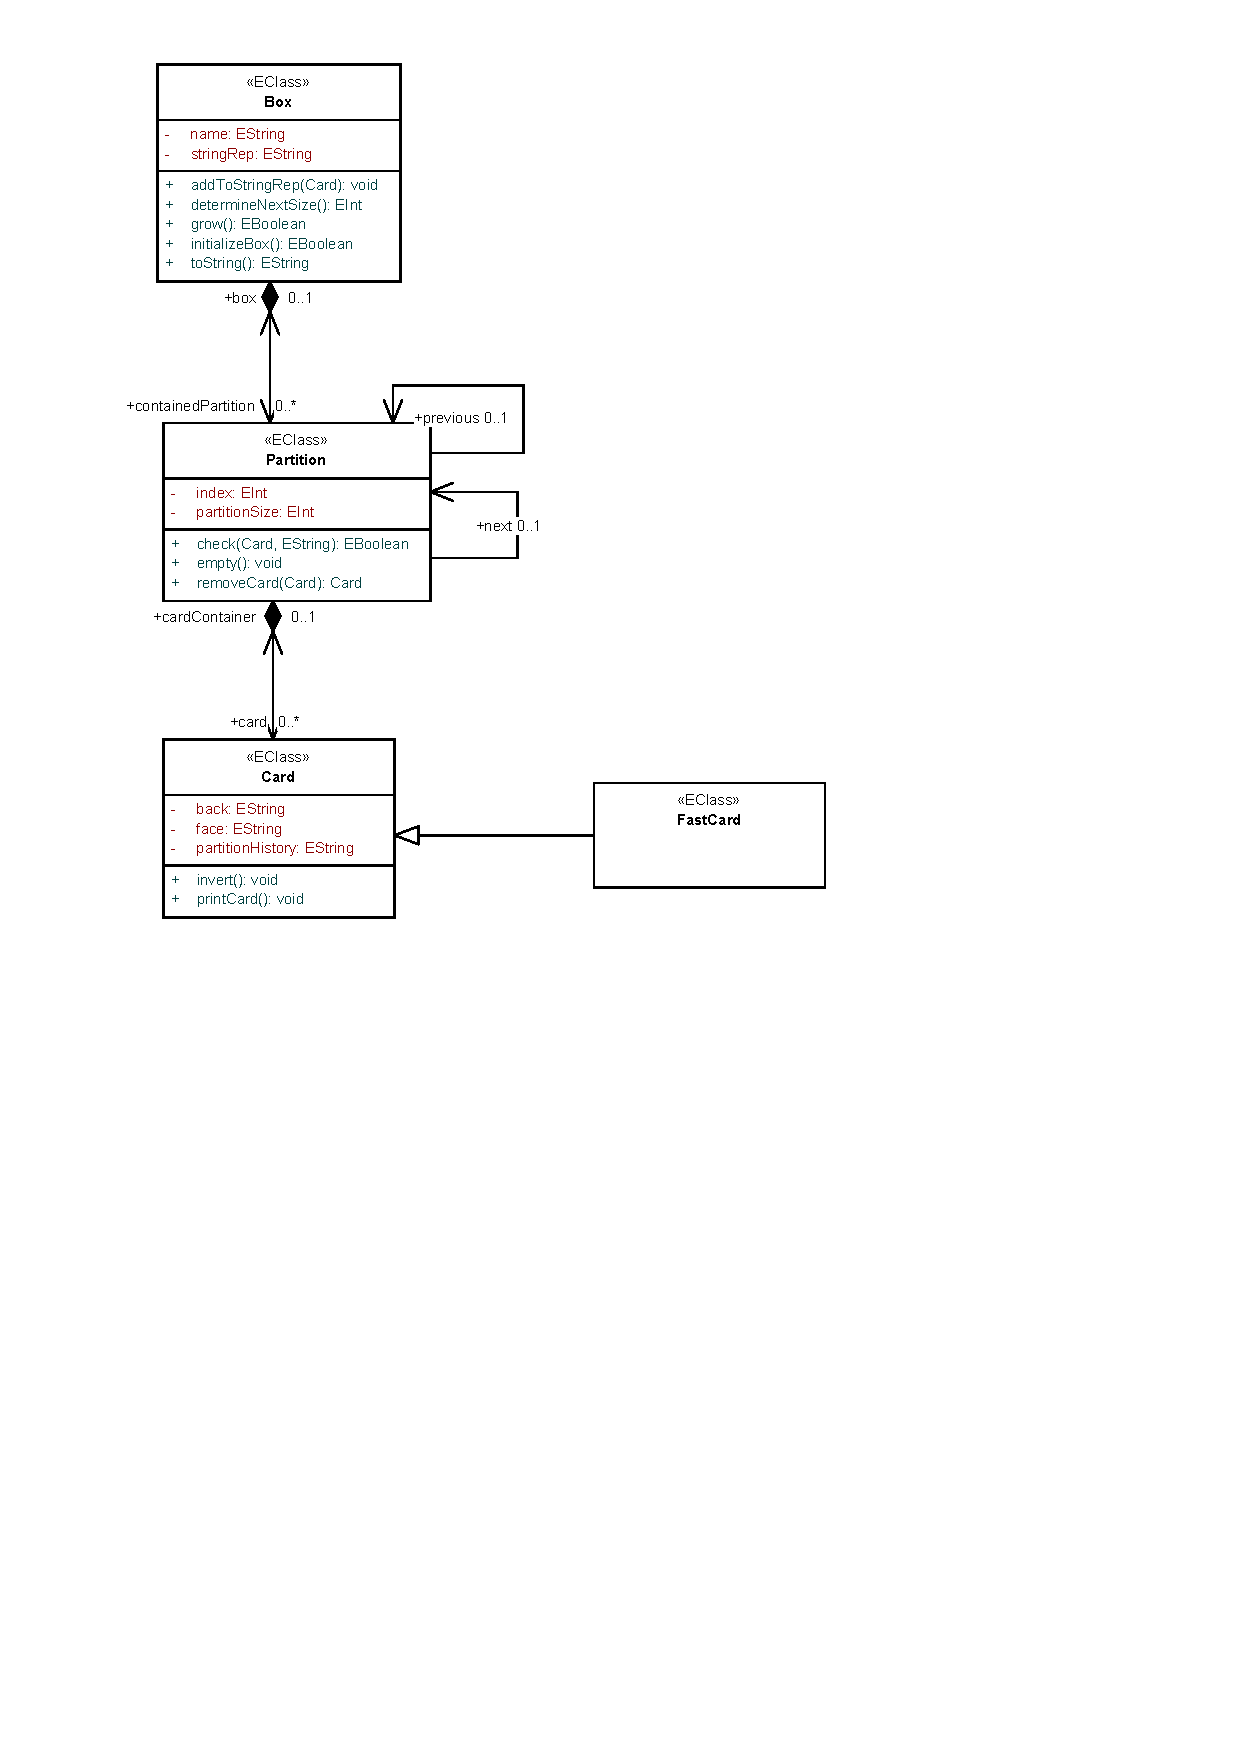
\includegraphics[width=1\textwidth]{LeitnersLearningBox_classdiagram}
	\caption{Classdiagram of \texttt{Learning\-Box\-Language}} 
	\label{ea:classdiagram_LearningBoxLanguage} 
\end{figure}